% Options for packages loaded elsewhere
\PassOptionsToPackage{unicode}{hyperref}
\PassOptionsToPackage{hyphens}{url}
%
\documentclass[
]{article}
\usepackage{amsmath,amssymb}
\usepackage{iftex}
\ifPDFTeX
  \usepackage[T1]{fontenc}
  \usepackage[utf8]{inputenc}
  \usepackage{textcomp} % provide euro and other symbols
\else % if luatex or xetex
  \usepackage{unicode-math} % this also loads fontspec
  \defaultfontfeatures{Scale=MatchLowercase}
  \defaultfontfeatures[\rmfamily]{Ligatures=TeX,Scale=1}
\fi
\usepackage{lmodern}
\ifPDFTeX\else
  % xetex/luatex font selection
\fi
% Use upquote if available, for straight quotes in verbatim environments
\IfFileExists{upquote.sty}{\usepackage{upquote}}{}
\IfFileExists{microtype.sty}{% use microtype if available
  \usepackage[]{microtype}
  \UseMicrotypeSet[protrusion]{basicmath} % disable protrusion for tt fonts
}{}
\makeatletter
\@ifundefined{KOMAClassName}{% if non-KOMA class
  \IfFileExists{parskip.sty}{%
    \usepackage{parskip}
  }{% else
    \setlength{\parindent}{0pt}
    \setlength{\parskip}{6pt plus 2pt minus 1pt}}
}{% if KOMA class
  \KOMAoptions{parskip=half}}
\makeatother
\usepackage{xcolor}
\usepackage[margin=1in]{geometry}
\usepackage{color}
\usepackage{fancyvrb}
\newcommand{\VerbBar}{|}
\newcommand{\VERB}{\Verb[commandchars=\\\{\}]}
\DefineVerbatimEnvironment{Highlighting}{Verbatim}{commandchars=\\\{\}}
% Add ',fontsize=\small' for more characters per line
\usepackage{framed}
\definecolor{shadecolor}{RGB}{248,248,248}
\newenvironment{Shaded}{\begin{snugshade}}{\end{snugshade}}
\newcommand{\AlertTok}[1]{\textcolor[rgb]{0.94,0.16,0.16}{#1}}
\newcommand{\AnnotationTok}[1]{\textcolor[rgb]{0.56,0.35,0.01}{\textbf{\textit{#1}}}}
\newcommand{\AttributeTok}[1]{\textcolor[rgb]{0.13,0.29,0.53}{#1}}
\newcommand{\BaseNTok}[1]{\textcolor[rgb]{0.00,0.00,0.81}{#1}}
\newcommand{\BuiltInTok}[1]{#1}
\newcommand{\CharTok}[1]{\textcolor[rgb]{0.31,0.60,0.02}{#1}}
\newcommand{\CommentTok}[1]{\textcolor[rgb]{0.56,0.35,0.01}{\textit{#1}}}
\newcommand{\CommentVarTok}[1]{\textcolor[rgb]{0.56,0.35,0.01}{\textbf{\textit{#1}}}}
\newcommand{\ConstantTok}[1]{\textcolor[rgb]{0.56,0.35,0.01}{#1}}
\newcommand{\ControlFlowTok}[1]{\textcolor[rgb]{0.13,0.29,0.53}{\textbf{#1}}}
\newcommand{\DataTypeTok}[1]{\textcolor[rgb]{0.13,0.29,0.53}{#1}}
\newcommand{\DecValTok}[1]{\textcolor[rgb]{0.00,0.00,0.81}{#1}}
\newcommand{\DocumentationTok}[1]{\textcolor[rgb]{0.56,0.35,0.01}{\textbf{\textit{#1}}}}
\newcommand{\ErrorTok}[1]{\textcolor[rgb]{0.64,0.00,0.00}{\textbf{#1}}}
\newcommand{\ExtensionTok}[1]{#1}
\newcommand{\FloatTok}[1]{\textcolor[rgb]{0.00,0.00,0.81}{#1}}
\newcommand{\FunctionTok}[1]{\textcolor[rgb]{0.13,0.29,0.53}{\textbf{#1}}}
\newcommand{\ImportTok}[1]{#1}
\newcommand{\InformationTok}[1]{\textcolor[rgb]{0.56,0.35,0.01}{\textbf{\textit{#1}}}}
\newcommand{\KeywordTok}[1]{\textcolor[rgb]{0.13,0.29,0.53}{\textbf{#1}}}
\newcommand{\NormalTok}[1]{#1}
\newcommand{\OperatorTok}[1]{\textcolor[rgb]{0.81,0.36,0.00}{\textbf{#1}}}
\newcommand{\OtherTok}[1]{\textcolor[rgb]{0.56,0.35,0.01}{#1}}
\newcommand{\PreprocessorTok}[1]{\textcolor[rgb]{0.56,0.35,0.01}{\textit{#1}}}
\newcommand{\RegionMarkerTok}[1]{#1}
\newcommand{\SpecialCharTok}[1]{\textcolor[rgb]{0.81,0.36,0.00}{\textbf{#1}}}
\newcommand{\SpecialStringTok}[1]{\textcolor[rgb]{0.31,0.60,0.02}{#1}}
\newcommand{\StringTok}[1]{\textcolor[rgb]{0.31,0.60,0.02}{#1}}
\newcommand{\VariableTok}[1]{\textcolor[rgb]{0.00,0.00,0.00}{#1}}
\newcommand{\VerbatimStringTok}[1]{\textcolor[rgb]{0.31,0.60,0.02}{#1}}
\newcommand{\WarningTok}[1]{\textcolor[rgb]{0.56,0.35,0.01}{\textbf{\textit{#1}}}}
\usepackage{longtable,booktabs,array}
\usepackage{calc} % for calculating minipage widths
% Correct order of tables after \paragraph or \subparagraph
\usepackage{etoolbox}
\makeatletter
\patchcmd\longtable{\par}{\if@noskipsec\mbox{}\fi\par}{}{}
\makeatother
% Allow footnotes in longtable head/foot
\IfFileExists{footnotehyper.sty}{\usepackage{footnotehyper}}{\usepackage{footnote}}
\makesavenoteenv{longtable}
\usepackage{graphicx}
\makeatletter
\def\maxwidth{\ifdim\Gin@nat@width>\linewidth\linewidth\else\Gin@nat@width\fi}
\def\maxheight{\ifdim\Gin@nat@height>\textheight\textheight\else\Gin@nat@height\fi}
\makeatother
% Scale images if necessary, so that they will not overflow the page
% margins by default, and it is still possible to overwrite the defaults
% using explicit options in \includegraphics[width, height, ...]{}
\setkeys{Gin}{width=\maxwidth,height=\maxheight,keepaspectratio}
% Set default figure placement to htbp
\makeatletter
\def\fps@figure{htbp}
\makeatother
\setlength{\emergencystretch}{3em} % prevent overfull lines
\providecommand{\tightlist}{%
  \setlength{\itemsep}{0pt}\setlength{\parskip}{0pt}}
\setcounter{secnumdepth}{-\maxdimen} % remove section numbering
\newlength{\cslhangindent}
\setlength{\cslhangindent}{1.5em}
\newlength{\csllabelwidth}
\setlength{\csllabelwidth}{3em}
\newlength{\cslentryspacingunit} % times entry-spacing
\setlength{\cslentryspacingunit}{\parskip}
\newenvironment{CSLReferences}[2] % #1 hanging-ident, #2 entry spacing
 {% don't indent paragraphs
  \setlength{\parindent}{0pt}
  % turn on hanging indent if param 1 is 1
  \ifodd #1
  \let\oldpar\par
  \def\par{\hangindent=\cslhangindent\oldpar}
  \fi
  % set entry spacing
  \setlength{\parskip}{#2\cslentryspacingunit}
 }%
 {}
\usepackage{calc}
\newcommand{\CSLBlock}[1]{#1\hfill\break}
\newcommand{\CSLLeftMargin}[1]{\parbox[t]{\csllabelwidth}{#1}}
\newcommand{\CSLRightInline}[1]{\parbox[t]{\linewidth - \csllabelwidth}{#1}\break}
\newcommand{\CSLIndent}[1]{\hspace{\cslhangindent}#1}
\ifLuaTeX
  \usepackage{selnolig}  % disable illegal ligatures
\fi
\IfFileExists{bookmark.sty}{\usepackage{bookmark}}{\usepackage{hyperref}}
\IfFileExists{xurl.sty}{\usepackage{xurl}}{} % add URL line breaks if available
\urlstyle{same}
\hypersetup{
  pdftitle={Introduction to Statistics and R for Neuroscience},
  hidelinks,
  pdfcreator={LaTeX via pandoc}}

\title{Introduction to Statistics and R for Neuroscience}
\author{}
\date{\vspace{-2.5em}}

\begin{document}
\maketitle

{
\setcounter{tocdepth}{2}
\tableofcontents
}
\hypertarget{introduction}{%
\section{Introduction}\label{introduction}}

The rapid advancement of neuroimaging technologies and high-performance
computing (HPC) has enabled neuroscience researchers to collect
unprecedented amounts of brain data, often referred to as ``big brain
data.'' This wealth of information allows scientists to revisit
longstanding questions and explore new ones on a much larger scale.
Indeed, there is, especially in neuroscience, a increasing demand for
novel statistical tools. Statisticians play a vital role in this
process, not only by developing models to analyze and interpret data but
also by incorporating biological insights into these frameworks, making
them more reflective of the underlying neural processes.

The impact of statistics on human neuroscience can be discussed through
the three main concepts of statistics defined by Ronald Fisher, father
of modern statistics:

\begin{itemize}
\tightlist
\item
  the study of populations,
\item
  the analysis of variance,
\item
  data reduction.
\end{itemize}

These foundational principles are central to key areas of brain
research, such as understanding connectivity between brain regions,
modeling the flow of information within and between areas, and
extracting meaningful patterns from large-scale neuroimaging data. For
example, predictive models are now frequently employed to anticipate
disease progression or classify patients based on brain features.

\hypertarget{study-of-populations}{%
\paragraph{Study of populations}\label{study-of-populations}}

Neuroscience research often involves three types of populations:

\begin{itemize}
\tightlist
\item
  population across individuals,
\item
  population across time,
\item
  population across brain regions.
\end{itemize}

Imagine scanning the brains of 100 individuals in an MRI scanner on a
single day. Here, the population is formed by the aggregate data across
these subjects, capturing inter-individual variability. If we scan one
individual every day for a year, the population shifts to reflect
temporal changes in the same person's brain over time. Finally, if we
examine connections across multiple regions within a single brain, the
population arises from spatial variability.

\hypertarget{analysis-of-variance}{%
\paragraph{Analysis of variance}\label{analysis-of-variance}}

Each of these populations introduces different types of
variance--between individuals, across time, or spatial--all of which
require tailored statistical methods to understand and quantify.

\hypertarget{data-reduction}{%
\paragraph{Data reduction}\label{data-reduction}}

One of the challenges in neuroscience is dealing with the scale of the
data. Data sets often contain hundreds of terabytes or even petabytes of
information, which, though rich in detail, can be noisy. Summarizing
this data effectively is critical for ensuring that statistical models
and computational tools can handle it efficiently. Moreover, the brain
itself provides a fascinating model for how to manage complexity: it
distills ever-changing sensory inputs into stable, universal patterns,
such as color or motion perception. Inspired by this, statisticians aim
to extract smaller, representative data sets that capture key patterns
across individuals or regions, distinguish healthy subjects from
patients, and track changes in mental states or disease progression over
time.

\hypertarget{statistical-integration-in-neuroscience}{%
\subsubsection{Statistical integration in
Neuroscience}\label{statistical-integration-in-neuroscience}}

Predictive modeling offers exciting opportunities in neuroscience,
enabling applications such as brain disease diagnosis and decoding
mental states. However, it also brings challenges, especially with
causal inference. Causal inference aims to determine whether an observed
relationship between two variables reflects a true cause-and-effect
relationship. For example, irregular neural signals in a specific brain
region may correlate with a mental disorder, but this association does
not necessarily imply causation. These signals could be an effect of the
disorder, or the relationship could arise from a coincidental
correlation caused by unmeasured factors. This challenge is further
exacerbated in high-dimensional brain data, where spurious correlations
or incidental endogeneity---features unintentionally correlated with the
model's error terms---can violate critical assumptions and lead to
misleading conclusions.

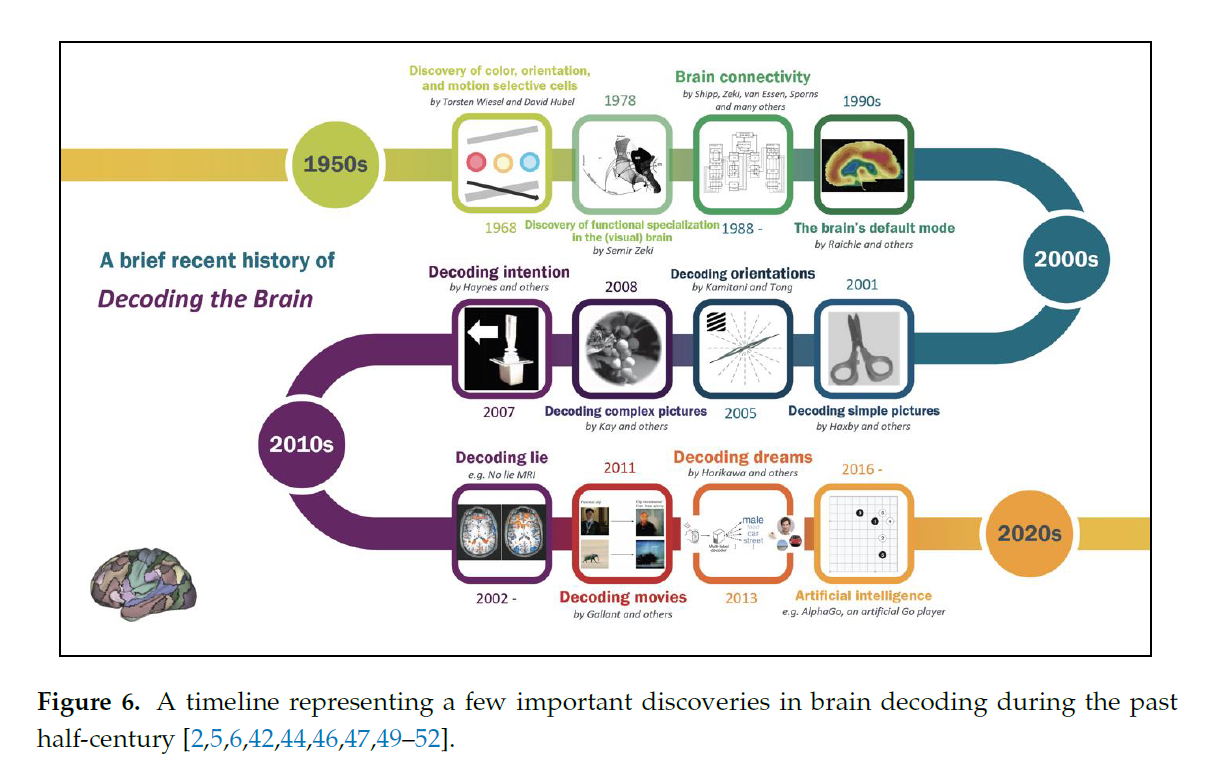
\includegraphics{stat_developments_history.png}

This figure provides a visual overview of how advancements in
neuroscience and statistical methods have evolved together to decode the
brain.

At its core, statistical inference allows researchers to generalize
findings from a small sample to a broader population. This process is
essential in neuroscience, where directly observing every aspect of the
brain is unfeasible. Careful attention to data validity and robustness
ensures that these generalizations are meaningful and scientifically
sound.\\
For instance, consider a study of a neuron's firing rate. Researchers
may relate this activity to an animal's position in a spatial
environment, its running speed, or the luminance of a visual stimulus.
Similarly, the study of synaptic receptor roles---such as NMDA
(N-Methyl-D-Aspartate) or GABA (Gamma-aminobutyric acid) receptors in
the hippocampus---illuminates mechanisms underlying cognitive tasks like
spatial learning. These examples illustrate how statistical inference
connects observations from experiments to theoretical understanding of
brain function.\\

The integration of statistical analysis, computer science technologies
and brain studies is advancing our understanding of brain function and
inspiring brain-like computers. Neural networks, for instance, are
designed following the structure and operation of the brain. McCulloch
and Pitts laid the groundwork for artificial neural networks by
conceptualizing a logical calculus for neural activity, framing the
brain as a computational device. Similarly, Hebb's rule, often
summarized as ``neurons that fire together, wire together,'' provided a
biological basis for learning mechanisms, influencing the design of
Rosenblatt's perceptron---the first artificial neural network capable of
performing simple tasks. Many neural network-based model have begun to
outperform humans in certain tasks, such as AlphaGo which demonstrated
unprecedented strategic thinking playing chess. Despite these successes,
these models fail to fully replicate the brain's structures and
processes. The collaboration between statistics and neuroscience can
bridge this gap: neuroscientists need statistical models capable of
deciphering the brain's dynamic, while statisticians require deeper
insights into the nervous system to enhance the biological plausibility
of their models. This synthesis not only aids in understanding the
brain's inner workings but also bridges the gap between data and
discovery.

\hypertarget{introduction-to-r}{%
\section{Introduction to R}\label{introduction-to-r}}

\hypertarget{what-is-r}{%
\paragraph{What is R}\label{what-is-r}}

R is a programming language that includes conditionals, loops, and the
ability to define custom functions allowing data processing and
graphical representation in the statistical domain. R serves as an
environment where various statistical techniques are implemented and
made available as \emph{packages}. Approximately 25 packages are
included in the base \texttt{R} environment, referred to as ``standard''
and ``recommended.'' All other packages are available through the R CRAN
website: \url{https://cran.r-project.org/}.

\hypertarget{why-use-r}{%
\paragraph{Why Use R:}\label{why-use-r}}

\begin{itemize}
\tightlist
\item
  Free software, available for download at the link above;
\item
  Available for multiple platforms (Windows, Linux, Macintosh);
\item
  Constantly developed and improved;
\item
  Versatile, allowing the development of new procedures.
\end{itemize}

It is possible to interact with R using \textbf{RStudio} (available at
\url{https://rstudio.com/}). RStudio allows users to write ``.R'' files
containing commands that can be executed in the R command prompt.
Additionally, it provides faster access to plots, the environment
(variables and functions defined during the session), and the help
documentation.

\hypertarget{rstudio-and-github}{%
\paragraph{Rstudio and GitHub}\label{rstudio-and-github}}

Git is an open-source version control system. It means that whenever a
developer develops some project (like an app) or something, he/she
constantly update it catering to the demands of users, technology, and
whatsoever it maybe. Version control systems keep these revisions
straight, storing the modifications in a central repository. It allows
developers to easily collaborate, as they can download a new version of
the software, make changes, and upload the newest revision. Every
developer can see these new changes, download them, and contribute. Git
is used to storing the source code for a project and track the complete
history of all changes to that code, while \textbf{GitHub} is a
cloud-based platform built around the Git tool.

It is possible to link a \emph{Rstudio project} to a \emph{GitHub
repository}. ~RStudio projects make it straightforward to divide your
work into multiple contexts, each with their own working directory,
workspace, history, and source documents. To create a new project in the
RStudio IDE, use the \texttt{New\ Project} command (available on the
\texttt{Projects} (top right corner) menu or go to
\texttt{File\ \textgreater{}\ New\ Project}. RStudio creates a project
file (with an \texttt{.Rproj} extension) within the project directory.
This file contains various project options and can also be used as a
shortcut for opening the project directly from the filesystem.

For more details:

\begin{itemize}
\tightlist
\item
  \url{https://rfortherestofus.com/2021/02/how-to-use-git-github-with-r/}
\item
  \url{https://annakrystalli.me/talks/r-in-repro-research.html\#27}
\end{itemize}

\hypertarget{rmarkdown}{%
\subsection{Rmarkdown}\label{rmarkdown}}

Rmarkdown (Xie, Allaire, and Grolemund 2018) is a powerful tool for
combining analysis and reporting into the same document. A complete
guide can be found at
\url{https://bookdown.org/yihui/rmarkdown-cookbook/}.\\
To use Rmarkdown we need to install the package \texttt{rmarkdown}

\begin{Shaded}
\begin{Highlighting}[]
\FunctionTok{install.packages}\NormalTok{(}\StringTok{"rmarkdown"}\NormalTok{)}
\end{Highlighting}
\end{Shaded}

A Rmarkdown \texttt{.Rmd} document has three components:

\begin{enumerate}
\def\labelenumi{\arabic{enumi}.}
\tightlist
\item
  \emph{yaml}: the document starts with yaml for setting metadata,
  e.g.~title, output format. You can also specify bibliography as
  \texttt{.bib} file (it must be in the same folder of the .Rmd file) or
  specify the full path where the .bib file is. For example, the yaml
  part of the current document is
\end{enumerate}

\begin{Shaded}
\begin{Highlighting}[]
\SpecialCharTok{{-}{-}{-}}
\NormalTok{title}\SpecialCharTok{:} \StringTok{"Introduction to Statistics and R for Neuroscience"}
\NormalTok{output}\SpecialCharTok{:}
\NormalTok{html\_document}\SpecialCharTok{:}
\NormalTok{    df\_print}\SpecialCharTok{:}\NormalTok{ paged}
\NormalTok{date}\SpecialCharTok{:} \StringTok{\textquotesingle{}\textquotesingle{}}
\NormalTok{bibliography}\SpecialCharTok{:}\NormalTok{ notes.bib}
\SpecialCharTok{{-}{-}{-}}
\end{Highlighting}
\end{Shaded}

Possible \texttt{output} formats include HTML, PDF, WORD, LaTeX.\\
2. \emph{text}: this is equivalent to writing in a text editor, but more
powerful and interesting for how the document is generated. Some simple
rules:

\begin{itemize}
\tightlist
\item
  Multiple spaces on a given line are reduced to one;
\item
  Line endings with fewer than two spaces are ignored;
\item
  Two or more spaces at the end of lines introduce hard breaks, forcing
  a new line;
\item
  Lines starting with the greater-than sign \textgreater{} introduce
  block quotes;
\item
  One or more blank lines introduce a new paragraph;
\item
  Text with the syntax
  \texttt{\textless{}!-\ -\ comments\ -\ -\ \textgreater{}} is omitted
  from output;
\item
  The sign \texttt{\#} introduces headers; lower levels are created with
  additional signs - up to total five levels;
\item
  \texttt{*italics*} becomes \emph{italics};
\item
  \texttt{**bold**} becomes \textbf{bold};
\item
  \texttt{{[}see\ this\ website{]}(website\_url)} becomes
  \href{website_url}{see this website};
\item
  you can also insert inline equations between a pair of single dollar
  sign, e.g.~\texttt{\$E=mc\^{}2\$} is displayed as \(E=mc^2\);
\item
  Block equations go in between a pair of double dollar signs,
  e.g.~\texttt{\$\$E=mc\^{}2\$\$} \[E=mc^2\]
\item
  Lines starting with asterisk \(*\) as well as plus \(+\) or minus
  \(-\) signs introduce lists.
\end{itemize}

\begin{enumerate}
\def\labelenumi{\arabic{enumi}.}
\setcounter{enumi}{2}
\tightlist
\item
  \emph{code chunks}: portions where to insert some code, e.g.~for R
  script. A code chunk takes a language engine (R, Pyhton, \ldots), and
  a label, that can be used for navigating through error messages.
  Duplicated labels lead to errors during compilation. Some of the most
  used options:
\end{enumerate}

\begin{itemize}
\item
  \texttt{include\ =\ FALSE}: do not include the output;
\item
  \texttt{echo\ =\ FALSE}: do not print the code;
\item
  \texttt{warning\ =\ FALSE}: exclude the warning message;
\item
  \texttt{comment\ =\ FALSE}: exclude the comments;
\item
  \texttt{eval\ =\ FALSE}: do not run the code;
\item
  \texttt{out.height\ =\ 50\%,\ out.width\ =\ 50\%}: define the size of
  figures as they appear in the output document;
\item
  \texttt{fig.align="center"}: Define the alignment of figures - left,
  right, or center;
\item
  \texttt{fig.caption="my\ caption"}: Define the caption for figures.\\
  The complete list of options is available at
  \url{https://yihui.org/knitr/options}.\\
  It is possible to include a figure in a Rmarkdown document:
\item
  \texttt{!{[}Figure\ Caption{]}(figure.extension)} in the text;
\item
  \texttt{knitr::include\_graphics("Images/figure.extension")} in a code
  chuck;
\item
  directly using R functions in a code chuck.
\end{itemize}

\hypertarget{basics-concepts}{%
\subsection{Basics concepts}\label{basics-concepts}}

For a detailed introduction to R sintax and commands please see the book
(Long and Teetor 2019) or the Supplemental material with code examples
and exercises of the \href{https://rc2e.com/}{R cookbook}.

R has a very simple syntax. It is \emph{case sensitive}, meaning it
distinguishes between uppercase and lowercase letters. The basic
commands include \emph{assignments} and \emph{expressions}. When an
expression, consisting of certain operations, is written in the prompt,
it is interpreted as a command, executed, and its result is displayed
(unless specified otherwise) but immediately lost. After the expression
is executed, the result is stored in a variable and not displayed. For
example:

\begin{Shaded}
\begin{Highlighting}[]
\NormalTok{x }\OtherTok{\textless{}{-}} \DecValTok{2} \SpecialCharTok{+} \DecValTok{3}
\NormalTok{x}
\end{Highlighting}
\end{Shaded}

\begin{verbatim}
## [1] 5
\end{verbatim}

In this case, we need to explicitly request the value to display it.\\
Commands can be separated by a semicolon (;) if written on the same
line. Otherwise, a newline is sufficient. While using semicolons reduces
the number of lines, it is discouraged as it affects code readability.

To obtain more information about any function, you can use the help
command. For example, to learn about the mean function:

\begin{Shaded}
\begin{Highlighting}[]
\FunctionTok{help}\NormalTok{(mean)}
\end{Highlighting}
\end{Shaded}

or alternatively \texttt{?mean}. Comments can be added to the code using
the \texttt{\#} symbol. Everything following the \texttt{\#} until the
end of the line is considered a comment.

Basic mathematical operations for addition, subtraction, multiplication,
and division use the standard symbols \(+\), \(-\), \(*\), and \(/\).
For exponentiation, use \(**\) or \^{}. The output of a command is
preceded by an index enclosed in square brackets. For example:

\begin{Shaded}
\begin{Highlighting}[]
\DecValTok{2} \SpecialCharTok{+} \DecValTok{3} \SpecialCharTok{*} \DecValTok{4}
\end{Highlighting}
\end{Shaded}

\begin{verbatim}
## [1] 14
\end{verbatim}

Operations follow the standard order of operations.

The following table summarizes the comparison and logical operators in
R:

\begin{longtable}[]{@{}ll@{}}
\toprule\noalign{}
Operator & Description \\
\midrule\noalign{}
\endhead
\bottomrule\noalign{}
\endlastfoot
\textless{} & Less than \\
\textgreater{} & Greater than \\
\(\le\) & Less than or equal \\
\(\ge\) & Greater than or equal \\
\(==\) & Equal to \\
\(!=\) & Not equal to \\
\& & AND \\
! & NOT \\
\end{longtable}

These operators are primarily used to verify conditions in R. For
example

\begin{Shaded}
\begin{Highlighting}[]
\DecValTok{4} \SpecialCharTok{*} \DecValTok{2} \SpecialCharTok{==} \DecValTok{2}\SpecialCharTok{\^{}}\DecValTok{3}
\end{Highlighting}
\end{Shaded}

\begin{verbatim}
## [1] TRUE
\end{verbatim}

Note: In R, TRUE and FALSE are binary values where TRUE corresponds to 1
and FALSE to 0.

At the end of an R session, all created objects can be permanently saved
in a file with the .RData extension in the current directory. The
command history is saved in a .Rhistory file. When R restarts in the
same directory, the workspace and history are loaded automatically. It
is good practice to set the working directory at the start of a session
using \texttt{setwd()}

\begin{Shaded}
\begin{Highlighting}[]
\FunctionTok{setwd}\NormalTok{(}\StringTok{"C:/desired/directory"}\NormalTok{)}
\end{Highlighting}
\end{Shaded}

\hypertarget{types-of-objects}{%
\subsection{Types of objects}\label{types-of-objects}}

\hypertarget{vectors}{%
\subsubsection{Vectors}\label{vectors}}

R operates on named data structures. The simplest type of structure is a
numeric vector, which is an ordered collection of numbers. You can
define a vector using the \texttt{c()} (concatenate) command as follows

\begin{Shaded}
\begin{Highlighting}[]
\NormalTok{x }\OtherTok{\textless{}{-}} \FunctionTok{c}\NormalTok{(}\DecValTok{1}\NormalTok{, }\DecValTok{2}\NormalTok{, }\DecValTok{3}\NormalTok{, }\DecValTok{4}\NormalTok{)}
\NormalTok{x}
\end{Highlighting}
\end{Shaded}

\begin{verbatim}
## [1] 1 2 3 4
\end{verbatim}

Here, we have created a vector with 4 elements. Note that the assignment
operator \texttt{\textless{}-} points directly to the object receiving
the assignment. Alternatively, the \(=\) symbol can be used. Assignments
can also be written in the reverse direction

\begin{Shaded}
\begin{Highlighting}[]
\FunctionTok{c}\NormalTok{(}\DecValTok{1}\NormalTok{, }\DecValTok{2}\NormalTok{, }\DecValTok{3}\NormalTok{, }\DecValTok{4}\NormalTok{) }\OtherTok{{-}\textgreater{}}\NormalTok{ x}
\end{Highlighting}
\end{Shaded}

You can also define a new vector by concatenating existing ones

\begin{Shaded}
\begin{Highlighting}[]
\NormalTok{y }\OtherTok{\textless{}{-}} \FunctionTok{c}\NormalTok{(x, }\DecValTok{0}\NormalTok{, x)}
\end{Highlighting}
\end{Shaded}

In this case, we create a vector of 9 elements by concatenating x, 0,
and x again. To determine the length of a vector, use the
\texttt{length()} function:

\begin{Shaded}
\begin{Highlighting}[]
\FunctionTok{length}\NormalTok{(y)}
\end{Highlighting}
\end{Shaded}

\begin{verbatim}
## [1] 9
\end{verbatim}

\hypertarget{arithmetic-operations-on-vectors}{%
\paragraph{Arithmetic Operations on
Vectors}\label{arithmetic-operations-on-vectors}}

Operations between vectors are performed element by element. Vectors
involved in an operation do not necessarily need to have the same
length. If they differ, the shorter vector is recycled until it matches
the length of the longer one. For example:

\begin{Shaded}
\begin{Highlighting}[]
\NormalTok{v }\OtherTok{\textless{}{-}} \DecValTok{2} \SpecialCharTok{*}\NormalTok{ x }\SpecialCharTok{+}\NormalTok{ y}
\end{Highlighting}
\end{Shaded}

\begin{verbatim}
## Warning in 2 * x + y: la lunghezza più lunga dell'oggetto non è un multiplo
## della lunghezza più corta dell'oggetto
\end{verbatim}

\begin{Shaded}
\begin{Highlighting}[]
\NormalTok{v}
\end{Highlighting}
\end{Shaded}

\begin{verbatim}
## [1]  3  6  9 12  2  5  8 11  6
\end{verbatim}

Note: If the lengths of the vectors are not multiples of each other, R
will still perform the operation but issue a warning.

In addition to basic arithmetic operations, there are commands for
specific mathematical functions, such as \texttt{log} for logarithm,
\texttt{sqrt} for square root, \texttt{exp} for exponential,
\texttt{sin} for sine, \texttt{cos} for cosine, and \texttt{abs} for
absolute value. Given a vector \texttt{x}, \texttt{min(x)} and
\texttt{max(x)} return the smallest and largest values, respectively.
The function \texttt{range(x)} returns a vector of length 2 with the
minimum and maximum values. \texttt{sum(x)} and \texttt{prod(x)} return
the sum and product of the elements of \texttt{x}, respectively. Lastly,
the function \texttt{sort(x)} returns a vector of the same length as
\texttt{x} sorted in ascending order.

\hypertarget{sequences}{%
\paragraph{Sequences}\label{sequences}}

R can easily generate sequences of numbers. For example

\begin{Shaded}
\begin{Highlighting}[]
\DecValTok{1}\SpecialCharTok{:}\DecValTok{10}
\end{Highlighting}
\end{Shaded}

\begin{verbatim}
##  [1]  1  2  3  4  5  6  7  8  9 10
\end{verbatim}

The colon operator has precedence over other operations. For instance,
to generate the first 10 even numbers, you can use

\begin{Shaded}
\begin{Highlighting}[]
\DecValTok{2} \SpecialCharTok{*} \DecValTok{1}\SpecialCharTok{:}\DecValTok{10}
\end{Highlighting}
\end{Shaded}

\begin{verbatim}
##  [1]  2  4  6  8 10 12 14 16 18 20
\end{verbatim}

You can also create descending sequences

\begin{Shaded}
\begin{Highlighting}[]
\DecValTok{10}\SpecialCharTok{:}\DecValTok{1}
\end{Highlighting}
\end{Shaded}

\begin{verbatim}
##  [1] 10  9  8  7  6  5  4  3  2  1
\end{verbatim}

To create sequences with a specific step size or length, use the
\texttt{seq()} function. For example

\begin{Shaded}
\begin{Highlighting}[]
\NormalTok{s1 }\OtherTok{\textless{}{-}} \FunctionTok{seq}\NormalTok{(}\SpecialCharTok{{-}}\DecValTok{1}\NormalTok{, }\DecValTok{1}\NormalTok{, }\AttributeTok{by =} \FloatTok{0.2}\NormalTok{)}
\NormalTok{s1}
\end{Highlighting}
\end{Shaded}

\begin{verbatim}
##  [1] -1.0 -0.8 -0.6 -0.4 -0.2  0.0  0.2  0.4  0.6  0.8  1.0
\end{verbatim}

\begin{Shaded}
\begin{Highlighting}[]
\NormalTok{s2 }\OtherTok{\textless{}{-}} \FunctionTok{seq}\NormalTok{(}\DecValTok{0}\NormalTok{, }\DecValTok{2}\NormalTok{, }\AttributeTok{length.out =} \DecValTok{5}\NormalTok{)}
\NormalTok{s2}
\end{Highlighting}
\end{Shaded}

\begin{verbatim}
## [1] 0.0 0.5 1.0 1.5 2.0
\end{verbatim}

\hypertarget{selecting-and-modifying-parts-of-a-vector}{%
\paragraph{Selecting and Modifying Parts of a
Vector}\label{selecting-and-modifying-parts-of-a-vector}}

You can select a subset of a vector using square brackets
\texttt{{[}{]}}. The content inside the brackets specifies the indices
to extract or modify. Common methods include:

\begin{Shaded}
\begin{Highlighting}[]
\NormalTok{y}
\end{Highlighting}
\end{Shaded}

\begin{verbatim}
## [1] 1 2 3 4 0 1 2 3 4
\end{verbatim}

\begin{Shaded}
\begin{Highlighting}[]
\CommentTok{\# extract first element}
\NormalTok{y[}\DecValTok{1}\NormalTok{]}
\end{Highlighting}
\end{Shaded}

\begin{verbatim}
## [1] 1
\end{verbatim}

\begin{Shaded}
\begin{Highlighting}[]
\CommentTok{\# extract elements from position 3 to 6}
\NormalTok{y[}\DecValTok{3}\SpecialCharTok{:}\DecValTok{6}\NormalTok{]}
\end{Highlighting}
\end{Shaded}

\begin{verbatim}
## [1] 3 4 0 1
\end{verbatim}

\begin{Shaded}
\begin{Highlighting}[]
\CommentTok{\# extract element in positions 2, 4, 8}
\NormalTok{y[}\FunctionTok{c}\NormalTok{(}\DecValTok{2}\NormalTok{, }\DecValTok{4}\NormalTok{, }\DecValTok{8}\NormalTok{)]}
\end{Highlighting}
\end{Shaded}

\begin{verbatim}
## [1] 2 4 3
\end{verbatim}

We can excludes elements at the specified positions

\begin{Shaded}
\begin{Highlighting}[]
\NormalTok{y[}\SpecialCharTok{{-}}\NormalTok{(}\DecValTok{1}\SpecialCharTok{:}\DecValTok{4}\NormalTok{)]}
\end{Highlighting}
\end{Shaded}

\begin{verbatim}
## [1] 0 1 2 3 4
\end{verbatim}

or selects elements which satisfy a certain condition (corresponding to
TRUE)

\begin{Shaded}
\begin{Highlighting}[]
\NormalTok{y[y }\SpecialCharTok{\textgreater{}} \DecValTok{2}\NormalTok{]}
\end{Highlighting}
\end{Shaded}

\begin{verbatim}
## [1] 3 4 3 4
\end{verbatim}

You can also modify elements of a vector by assigning new values:

\begin{Shaded}
\begin{Highlighting}[]
\NormalTok{y[y }\SpecialCharTok{==} \DecValTok{1}\NormalTok{] }\OtherTok{\textless{}{-}} \SpecialCharTok{{-}}\DecValTok{2}
\NormalTok{y}
\end{Highlighting}
\end{Shaded}

\begin{verbatim}
## [1] -2  2  3  4  0 -2  2  3  4
\end{verbatim}

\hypertarget{matrices}{%
\subsubsection{Matrices}\label{matrices}}

In general, a matrix is a two-dimensional generalization of a vector.
The base function to create a matrix is \texttt{matrix()}. If no
arguments are provided, a matrix with a single column is created:

\begin{Shaded}
\begin{Highlighting}[]
\FunctionTok{matrix}\NormalTok{(}\DecValTok{1}\SpecialCharTok{:}\DecValTok{5}\NormalTok{)}
\end{Highlighting}
\end{Shaded}

\begin{verbatim}
##      [,1]
## [1,]    1
## [2,]    2
## [3,]    3
## [4,]    4
## [5,]    5
\end{verbatim}

Note that this is not equivalent to a column vector, as a second
dimension is still defined. The indices shown in the output indicate the
row and column of the element within the matrix. To create a matrix with
specific dimensions, you need to specify them:

\begin{Shaded}
\begin{Highlighting}[]
\FunctionTok{matrix}\NormalTok{(}\DecValTok{1}\SpecialCharTok{:}\DecValTok{6}\NormalTok{, }\AttributeTok{nrow =} \DecValTok{2}\NormalTok{)}
\end{Highlighting}
\end{Shaded}

\begin{verbatim}
##      [,1] [,2] [,3]
## [1,]    1    3    5
## [2,]    2    4    6
\end{verbatim}

By default, matrices are filled column-wise. To fill them row-wise, use
the \texttt{byrow\ =\ TRUE} argument:

\begin{Shaded}
\begin{Highlighting}[]
\FunctionTok{matrix}\NormalTok{(}\DecValTok{1}\SpecialCharTok{:}\DecValTok{6}\NormalTok{, }\AttributeTok{nrow =} \DecValTok{2}\NormalTok{, }\AttributeTok{byrow =} \ConstantTok{TRUE}\NormalTok{)}
\end{Highlighting}
\end{Shaded}

\begin{verbatim}
##      [,1] [,2] [,3]
## [1,]    1    2    3
## [2,]    4    5    6
\end{verbatim}

You can also specify the number of columns using the \texttt{ncol}
argument. Given a matrix \texttt{A}, you can determine its dimensions
using the \texttt{dim()} function, which returns a vector with the
number of rows and columns.

\hypertarget{constructing-matrices-from-existing-vectors}{%
\paragraph{Constructing Matrices from Existing
Vectors}\label{constructing-matrices-from-existing-vectors}}

A matrix can also be built from an existing vector. Consider the
following vector containing data on the area, population, and altitude
of three Italian cities:

\begin{Shaded}
\begin{Highlighting}[]
\NormalTok{dati }\OtherTok{\textless{}{-}} \FunctionTok{c}\NormalTok{(}\FloatTok{157.88}\NormalTok{, }\DecValTok{120709}\NormalTok{, }\DecValTok{194}\NormalTok{, }\FloatTok{52.29}\NormalTok{, }\DecValTok{107816}\NormalTok{, }\DecValTok{262}\NormalTok{, }\FloatTok{140.86}\NormalTok{, }\DecValTok{395149}\NormalTok{, }\DecValTok{54}\NormalTok{)}
\end{Highlighting}
\end{Shaded}

Using the \texttt{matrix} function, we can create the
\texttt{province\_dati} matrix:

\begin{Shaded}
\begin{Highlighting}[]
\NormalTok{province\_dati }\OtherTok{\textless{}{-}} \FunctionTok{matrix}\NormalTok{(dati, }\AttributeTok{nrow =} \DecValTok{3}\NormalTok{, }\AttributeTok{byrow =} \ConstantTok{TRUE}\NormalTok{)}
\NormalTok{province\_dati}
\end{Highlighting}
\end{Shaded}

\begin{verbatim}
##        [,1]   [,2] [,3]
## [1,] 157.88 120709  194
## [2,]  52.29 107816  262
## [3,] 140.86 395149   54
\end{verbatim}

\begin{Shaded}
\begin{Highlighting}[]
\FunctionTok{dim}\NormalTok{(province\_dati)}
\end{Highlighting}
\end{Shaded}

\begin{verbatim}
## [1] 3 3
\end{verbatim}

\hypertarget{naming-rows-and-columns}{%
\paragraph{Naming Rows and Columns}\label{naming-rows-and-columns}}

Row and column names can be assigned using the \texttt{rownames()} and
\texttt{colnames()} functions:

\begin{Shaded}
\begin{Highlighting}[]
\FunctionTok{rownames}\NormalTok{(province\_dati) }\OtherTok{\textless{}{-}} \FunctionTok{c}\NormalTok{(}\StringTok{"Trento"}\NormalTok{, }\StringTok{"Bolzano"}\NormalTok{, }\StringTok{"Bologna"}\NormalTok{)}
\FunctionTok{colnames}\NormalTok{(province\_dati) }\OtherTok{\textless{}{-}} \FunctionTok{c}\NormalTok{(}\StringTok{"Area"}\NormalTok{, }\StringTok{"Population"}\NormalTok{, }\StringTok{"Altitude"}\NormalTok{)}
\NormalTok{province\_dati}
\end{Highlighting}
\end{Shaded}

\begin{verbatim}
##           Area Population Altitude
## Trento  157.88     120709      194
## Bolzano  52.29     107816      262
## Bologna 140.86     395149       54
\end{verbatim}

Alternatively, the \texttt{dimnames()} function can be used to assign
both row and column names simultaneously

\begin{Shaded}
\begin{Highlighting}[]
\FunctionTok{dimnames}\NormalTok{(province\_dati) }\OtherTok{\textless{}{-}} \FunctionTok{list}\NormalTok{(}\FunctionTok{c}\NormalTok{(}\StringTok{"Trento"}\NormalTok{, }\StringTok{"Bolzano"}\NormalTok{, }\StringTok{"Bologna"}\NormalTok{), }
                                  \FunctionTok{c}\NormalTok{(}\StringTok{"Area"}\NormalTok{, }\StringTok{"Population"}\NormalTok{, }\StringTok{"Altitude"}\NormalTok{))}
\end{Highlighting}
\end{Shaded}

To retrieve row or column names without assigning new ones

\begin{Shaded}
\begin{Highlighting}[]
\FunctionTok{colnames}\NormalTok{(province\_dati)}
\end{Highlighting}
\end{Shaded}

\begin{verbatim}
## [1] "Area"       "Population" "Altitude"
\end{verbatim}

\begin{Shaded}
\begin{Highlighting}[]
\FunctionTok{dimnames}\NormalTok{(province\_dati)}
\end{Highlighting}
\end{Shaded}

\begin{verbatim}
## [[1]]
## [1] "Trento"  "Bolzano" "Bologna"
## 
## [[2]]
## [1] "Area"       "Population" "Altitude"
\end{verbatim}

\hypertarget{accessing-matrix-elements}{%
\paragraph{Accessing Matrix Elements}\label{accessing-matrix-elements}}

To access specific elements of a matrix, use square brackets
\texttt{{[}row,\ column{]}}. For example, to retrieve the population of
Trento (row 1, column 2):

\begin{Shaded}
\begin{Highlighting}[]
\NormalTok{province\_dati[}\DecValTok{1}\NormalTok{, }\DecValTok{2}\NormalTok{]}
\end{Highlighting}
\end{Shaded}

\begin{verbatim}
## [1] 120709
\end{verbatim}

To retrieve all data for Bolzano (row 2):

\begin{Shaded}
\begin{Highlighting}[]
\NormalTok{province\_dati[}\DecValTok{2}\NormalTok{, ]}
\end{Highlighting}
\end{Shaded}

\begin{verbatim}
##       Area Population   Altitude 
##      52.29  107816.00     262.00
\end{verbatim}

You can also use row and column names for indexing:

\begin{Shaded}
\begin{Highlighting}[]
\NormalTok{province\_dati[}\StringTok{"Bologna"}\NormalTok{, }\StringTok{"Area"}\NormalTok{]}
\end{Highlighting}
\end{Shaded}

\begin{verbatim}
## [1] 140.86
\end{verbatim}

\hypertarget{operations-on-matrices}{%
\paragraph{Operations on Matrices}\label{operations-on-matrices}}

Matrices support element-wise operations such as addition, subtraction,
multiplication, and division. Consider the following matrices

\begin{Shaded}
\begin{Highlighting}[]
\NormalTok{A }\OtherTok{\textless{}{-}} \FunctionTok{matrix}\NormalTok{(}\DecValTok{0}\SpecialCharTok{:}\DecValTok{5}\NormalTok{, }\AttributeTok{nrow =} \DecValTok{2}\NormalTok{, }\AttributeTok{ncol =} \DecValTok{3}\NormalTok{)}
\NormalTok{B }\OtherTok{\textless{}{-}} \FunctionTok{matrix}\NormalTok{(}\FunctionTok{seq}\NormalTok{(}\DecValTok{0}\NormalTok{, }\DecValTok{10}\NormalTok{, }\DecValTok{2}\NormalTok{), }\AttributeTok{nrow =} \DecValTok{2}\NormalTok{, }\AttributeTok{ncol =} \DecValTok{3}\NormalTok{)}
\end{Highlighting}
\end{Shaded}

Element-wise addition and subtraction:

\begin{Shaded}
\begin{Highlighting}[]
\NormalTok{A }\SpecialCharTok{+}\NormalTok{ B}
\end{Highlighting}
\end{Shaded}

\begin{verbatim}
##      [,1] [,2] [,3]
## [1,]    0    6   12
## [2,]    3    9   15
\end{verbatim}

\begin{Shaded}
\begin{Highlighting}[]
\NormalTok{A }\SpecialCharTok{{-}}\NormalTok{ B}
\end{Highlighting}
\end{Shaded}

\begin{verbatim}
##      [,1] [,2] [,3]
## [1,]    0   -2   -4
## [2,]   -1   -3   -5
\end{verbatim}

Element-wise multiplication and division:

\begin{Shaded}
\begin{Highlighting}[]
\NormalTok{A }\SpecialCharTok{*}\NormalTok{ B}
\end{Highlighting}
\end{Shaded}

\begin{verbatim}
##      [,1] [,2] [,3]
## [1,]    0    8   32
## [2,]    2   18   50
\end{verbatim}

\begin{Shaded}
\begin{Highlighting}[]
\NormalTok{A }\SpecialCharTok{/}\NormalTok{ B}
\end{Highlighting}
\end{Shaded}

\begin{verbatim}
##      [,1] [,2] [,3]
## [1,]  NaN  0.5  0.5
## [2,]  0.5  0.5  0.5
\end{verbatim}

Division by zero results in \texttt{NaN} (Not a Number), indicating
invalid numeric operations.

\hypertarget{adding-rows-and-columns}{%
\paragraph{Adding Rows and Columns}\label{adding-rows-and-columns}}

You can add rows or columns to an existing matrix using \texttt{rbind()}
and \texttt{cbind()}. For example, to add a column for population
density:

\begin{Shaded}
\begin{Highlighting}[]
\NormalTok{Density }\OtherTok{\textless{}{-}}\NormalTok{ province\_dati[, }\StringTok{"Population"}\NormalTok{] }\SpecialCharTok{/}\NormalTok{ province\_dati[, }\StringTok{"Area"}\NormalTok{]}
\NormalTok{Density }\OtherTok{\textless{}{-}} \FunctionTok{round}\NormalTok{(Density, }\AttributeTok{digits =} \DecValTok{2}\NormalTok{)}
\NormalTok{province\_dati }\OtherTok{\textless{}{-}} \FunctionTok{cbind}\NormalTok{(province\_dati, Density)}
\NormalTok{province\_dati}
\end{Highlighting}
\end{Shaded}

\begin{verbatim}
##           Area Population Altitude Density
## Trento  157.88     120709      194  764.56
## Bolzano  52.29     107816      262 2061.89
## Bologna 140.86     395149       54 2805.26
\end{verbatim}

To add a new row for another city:

\begin{Shaded}
\begin{Highlighting}[]
\NormalTok{Trapani }\OtherTok{\textless{}{-}} \FunctionTok{c}\NormalTok{(}\FloatTok{273.13}\NormalTok{, }\DecValTok{65431}\NormalTok{, }\DecValTok{3}\NormalTok{, }\FloatTok{239.56}\NormalTok{)}
\NormalTok{province\_dati }\OtherTok{\textless{}{-}} \FunctionTok{rbind}\NormalTok{(province\_dati, Trapani)}
\NormalTok{province\_dati}
\end{Highlighting}
\end{Shaded}

\begin{verbatim}
##           Area Population Altitude Density
## Trento  157.88     120709      194  764.56
## Bolzano  52.29     107816      262 2061.89
## Bologna 140.86     395149       54 2805.26
## Trapani 273.13      65431        3  239.56
\end{verbatim}

\hypertarget{multi-dimensional-arrays}{%
\subsubsection{Multi-Dimensional
Arrays}\label{multi-dimensional-arrays}}

Beyond matrices, R supports higher-dimensional arrays. For example:

\begin{Shaded}
\begin{Highlighting}[]
\NormalTok{x }\OtherTok{\textless{}{-}} \FunctionTok{array}\NormalTok{(}\DecValTok{1}\SpecialCharTok{:}\DecValTok{24}\NormalTok{, }\FunctionTok{c}\NormalTok{(}\DecValTok{3}\NormalTok{, }\DecValTok{4}\NormalTok{, }\DecValTok{2}\NormalTok{))}
\NormalTok{x}
\end{Highlighting}
\end{Shaded}

\begin{verbatim}
## , , 1
## 
##      [,1] [,2] [,3] [,4]
## [1,]    1    4    7   10
## [2,]    2    5    8   11
## [3,]    3    6    9   12
## 
## , , 2
## 
##      [,1] [,2] [,3] [,4]
## [1,]   13   16   19   22
## [2,]   14   17   20   23
## [3,]   15   18   21   24
\end{verbatim}

This creates a 3x4x2 array. Array dimensions and elements can be
accessed in a similar way to matrices.

\hypertarget{qualitative-variables-factor}{%
\subsubsection{Qualitative Variables
(Factor)}\label{qualitative-variables-factor}}

An object of type \texttt{factor} is used to indicate a discrete
classification (or grouping) of the elements in a vector of the same
length. For example, consider the data for the height of 30 individuals
whose gender is specified as:

\begin{Shaded}
\begin{Highlighting}[]
\NormalTok{genere }\OtherTok{\textless{}{-}} \FunctionTok{c}\NormalTok{(}\StringTok{"F"}\NormalTok{, }\StringTok{"M"}\NormalTok{, }\StringTok{"M"}\NormalTok{, }\StringTok{"F"}\NormalTok{, }\StringTok{"M"}\NormalTok{, }\StringTok{"F"}\NormalTok{, }\StringTok{"F"}\NormalTok{, }\StringTok{"F"}\NormalTok{, }\StringTok{"M"}\NormalTok{, }\StringTok{"F"}\NormalTok{, }
            \StringTok{"M"}\NormalTok{, }\StringTok{"M"}\NormalTok{, }\StringTok{"F"}\NormalTok{, }\StringTok{"F"}\NormalTok{, }\StringTok{"M"}\NormalTok{, }\StringTok{"M"}\NormalTok{, }\StringTok{"M"}\NormalTok{, }\StringTok{"F"}\NormalTok{, }\StringTok{"F"}\NormalTok{, }\StringTok{"M"}\NormalTok{)}
\end{Highlighting}
\end{Shaded}

A factor is created using the \texttt{factor()} function

\begin{Shaded}
\begin{Highlighting}[]
\NormalTok{generef }\OtherTok{\textless{}{-}} \FunctionTok{factor}\NormalTok{(genere)}
\NormalTok{generef}
\end{Highlighting}
\end{Shaded}

\begin{verbatim}
##  [1] F M M F M F F F M F M M F F M M M F F M
## Levels: F M
\end{verbatim}

Factors have a representation slightly different from vectors. They
include the possible \texttt{levels} that the variable can take. To
retrieve the levels of a factor

\begin{Shaded}
\begin{Highlighting}[]
\FunctionTok{levels}\NormalTok{(generef)}
\end{Highlighting}
\end{Shaded}

\begin{verbatim}
## [1] "F" "M"
\end{verbatim}

Continuing the example, consider the following height values for
individuals, expressed in centimeters

\begin{Shaded}
\begin{Highlighting}[]
\NormalTok{Altezza }\OtherTok{\textless{}{-}} \FunctionTok{c}\NormalTok{(}\FloatTok{145.1787}\NormalTok{, }\FloatTok{185.0102}\NormalTok{, }\FloatTok{195.1313}\NormalTok{, }\FloatTok{161.1447}\NormalTok{, }\FloatTok{186.5746}\NormalTok{, }\FloatTok{148.6862}\NormalTok{, }
             \FloatTok{166.3729}\NormalTok{, }\FloatTok{150.0860}\NormalTok{, }\FloatTok{175.6791}\NormalTok{, }\FloatTok{157.0512}\NormalTok{, }\FloatTok{167.5121}\NormalTok{, }\FloatTok{188.3428}\NormalTok{, }
             \FloatTok{152.6443}\NormalTok{, }\FloatTok{171.8734}\NormalTok{, }\FloatTok{181.6952}\NormalTok{, }\FloatTok{187.6279}\NormalTok{, }\FloatTok{200.6651}\NormalTok{, }\FloatTok{153.4996}\NormalTok{, }
             \FloatTok{163.1848}\NormalTok{, }\FloatTok{180.1263}\NormalTok{)}
\end{Highlighting}
\end{Shaded}

We can perform operations on this vector with respect to the levels of
the factor using the \texttt{tapply()} function

\begin{Shaded}
\begin{Highlighting}[]
\FunctionTok{tapply}\NormalTok{(Altezza, generef, mean)}
\end{Highlighting}
\end{Shaded}

\begin{verbatim}
##        F        M 
## 156.9722 184.8365
\end{verbatim}

Here, we computed the average height of individuals grouped by gender
(using the factor variable). The \texttt{tapply} function requires the
vector to operate on, a factor of the same length, and the function to
apply. The output displays the results labeled by the levels used.
Similarly, you can use the by() function:

\begin{Shaded}
\begin{Highlighting}[]
\FunctionTok{by}\NormalTok{(Altezza, generef, mean)}
\end{Highlighting}
\end{Shaded}

\begin{verbatim}
## generef: F
## [1] 156.9722
## ------------------------------------------------------------ 
## generef: M
## [1] 184.8365
\end{verbatim}

\hypertarget{ordered-factors}{%
\paragraph{Ordered Factors}\label{ordered-factors}}

By default, factor levels are sorted alphabetically. To specify a custom
order for the levels, use the levels argument within the factor()
function. For instance, consider a variable \texttt{Grado} representing
education levels with levels ordered as `S: diploma superiore'
\textless{} `L: laurea' \textless{} `D: dottorato':

\begin{Shaded}
\begin{Highlighting}[]
\NormalTok{Grado }\OtherTok{\textless{}{-}} \FunctionTok{c}\NormalTok{(}\StringTok{"S"}\NormalTok{, }\StringTok{"D"}\NormalTok{, }\StringTok{"D"}\NormalTok{, }\StringTok{"S"}\NormalTok{, }\StringTok{"D"}\NormalTok{, }\StringTok{"S"}\NormalTok{, }\StringTok{"L"}\NormalTok{, }\StringTok{"S"}\NormalTok{, }\StringTok{"S"}\NormalTok{, }\StringTok{"L"}\NormalTok{, }
           \StringTok{"S"}\NormalTok{, }\StringTok{"D"}\NormalTok{, }\StringTok{"S"}\NormalTok{, }\StringTok{"S"}\NormalTok{, }\StringTok{"L"}\NormalTok{, }\StringTok{"L"}\NormalTok{, }\StringTok{"S"}\NormalTok{, }\StringTok{"D"}\NormalTok{, }\StringTok{"D"}\NormalTok{, }\StringTok{"D"}\NormalTok{)}
\NormalTok{Grado}
\end{Highlighting}
\end{Shaded}

\begin{verbatim}
##  [1] "S" "D" "D" "S" "D" "S" "L" "S" "S" "L" "S" "D" "S" "S" "L" "L" "S" "D" "D"
## [20] "D"
\end{verbatim}

\begin{Shaded}
\begin{Highlighting}[]
\NormalTok{Gradof }\OtherTok{\textless{}{-}} \FunctionTok{factor}\NormalTok{(Grado, }\AttributeTok{levels =} \FunctionTok{c}\NormalTok{(}\StringTok{"S"}\NormalTok{, }\StringTok{"L"}\NormalTok{, }\StringTok{"D"}\NormalTok{), }\AttributeTok{ordered =} \ConstantTok{TRUE}\NormalTok{)}
\NormalTok{Gradof}
\end{Highlighting}
\end{Shaded}

\begin{verbatim}
##  [1] S D D S D S L S S L S D S S L L S D D D
## Levels: S < L < D
\end{verbatim}

Alternatively, you can use the ordered() function to create an ordered
factor:

\begin{Shaded}
\begin{Highlighting}[]
\FunctionTok{ordered}\NormalTok{(Grado, }\AttributeTok{levels =} \FunctionTok{c}\NormalTok{(}\StringTok{"S"}\NormalTok{, }\StringTok{"L"}\NormalTok{, }\StringTok{"D"}\NormalTok{))}
\end{Highlighting}
\end{Shaded}

\begin{verbatim}
##  [1] S D D S D S L S S L S D S S L L S D D D
## Levels: S < L < D
\end{verbatim}

\hypertarget{data-frames}{%
\subsubsection{Data Frames}\label{data-frames}}

Suppose we want to add a column to the matrix \texttt{province\_dati}
containing the corresponding province abbreviations

\begin{Shaded}
\begin{Highlighting}[]
\NormalTok{Sigla }\OtherTok{\textless{}{-}} \FunctionTok{c}\NormalTok{(}\StringTok{"TN"}\NormalTok{, }\StringTok{"BZ"}\NormalTok{, }\StringTok{"BO"}\NormalTok{, }\StringTok{"TP"}\NormalTok{)}
\end{Highlighting}
\end{Shaded}

Using the \texttt{cbind()} function, we can add this vector to the
matrix

\begin{Shaded}
\begin{Highlighting}[]
\NormalTok{province\_dati1 }\OtherTok{\textless{}{-}} \FunctionTok{cbind}\NormalTok{(province\_dati, Sigla)}
\NormalTok{province\_dati1}
\end{Highlighting}
\end{Shaded}

\begin{verbatim}
##         Area     Population Altitude Density   Sigla
## Trento  "157.88" "120709"   "194"    "764.56"  "TN" 
## Bolzano "52.29"  "107816"   "262"    "2061.89" "BZ" 
## Bologna "140.86" "395149"   "54"     "2805.26" "BO" 
## Trapani "273.13" "65431"    "3"      "239.56"  "TP"
\end{verbatim}

However, adding a column of strings converts all numeric vectors in the
matrix to strings (note the quotation marks). This happens because
arrays (of any dimension) can only contain objects of the same type. To
avoid this issue, we use data frames, which are similar to matrices but
can contain vectors of different types. Create a data frame with the
\texttt{data.frame()} function

\begin{Shaded}
\begin{Highlighting}[]
\NormalTok{province\_frame }\OtherTok{\textless{}{-}} \FunctionTok{data.frame}\NormalTok{(province\_dati, Sigla)}
\NormalTok{province\_frame}
\end{Highlighting}
\end{Shaded}

\begin{verbatim}
##           Area Population Altitude Density Sigla
## Trento  157.88     120709      194  764.56    TN
## Bolzano  52.29     107816      262 2061.89    BZ
## Bologna 140.86     395149       54 2805.26    BO
## Trapani 273.13      65431        3  239.56    TP
\end{verbatim}

Additionally, columns can be accessed directly using the \texttt{\$}
operator:

\begin{Shaded}
\begin{Highlighting}[]
\NormalTok{province\_frame[, }\DecValTok{3}\NormalTok{]}
\end{Highlighting}
\end{Shaded}

\begin{verbatim}
## [1] 194 262  54   3
\end{verbatim}

\begin{Shaded}
\begin{Highlighting}[]
\NormalTok{province\_frame}\SpecialCharTok{$}\NormalTok{Altitude}
\end{Highlighting}
\end{Shaded}

\begin{verbatim}
## [1] 194 262  54   3
\end{verbatim}

Alternatively, you can attach the data frame to make its columns
directly accessible by name

\begin{Shaded}
\begin{Highlighting}[]
\FunctionTok{attach}\NormalTok{(province\_frame)}
\NormalTok{Population}
\end{Highlighting}
\end{Shaded}

\begin{verbatim}
## [1] 120709 107816 395149  65431
\end{verbatim}

To remove direct access, use the \texttt{detach()} function:

\begin{Shaded}
\begin{Highlighting}[]
\FunctionTok{detach}\NormalTok{(province\_frame)}
\end{Highlighting}
\end{Shaded}

To get an overview of a data frame's structure, use the \texttt{str()}
function:

\begin{Shaded}
\begin{Highlighting}[]
\FunctionTok{str}\NormalTok{(province\_frame)}
\end{Highlighting}
\end{Shaded}

\begin{verbatim}
## 'data.frame':    4 obs. of  5 variables:
##  $ Area      : num  157.9 52.3 140.9 273.1
##  $ Population: num  120709 107816 395149 65431
##  $ Altitude  : num  194 262 54 3
##  $ Density   : num  765 2062 2805 240
##  $ Sigla     : chr  "TN" "BZ" "BO" "TP"
\end{verbatim}

\hypertarget{lists}{%
\subsubsection{Lists}\label{lists}}

Data frames generalize matrices, allowing operations on objects that can
include numeric vectors. A more flexible structure is the list, which
allows combining objects of different types and dimensions, such as
matrices, character vectors, and data frames. For example, given the
following elements

\begin{Shaded}
\begin{Highlighting}[]
\NormalTok{A }\OtherTok{\textless{}{-}} \FunctionTok{matrix}\NormalTok{(}\FunctionTok{c}\NormalTok{(}\DecValTok{1}\NormalTok{, }\DecValTok{0}\NormalTok{, }\DecValTok{0}\NormalTok{, }\DecValTok{1}\NormalTok{), }\AttributeTok{nrow =} \DecValTok{2}\NormalTok{)}
\NormalTok{regioni }\OtherTok{\textless{}{-}} \FunctionTok{c}\NormalTok{(}\StringTok{"Trentino{-}Alto Adige"}\NormalTok{, }\StringTok{"Emilia Romagna"}\NormalTok{, }\StringTok{"Sicilia"}\NormalTok{)}
\end{Highlighting}
\end{Shaded}

We can combine them into a single list:

\begin{Shaded}
\begin{Highlighting}[]
\NormalTok{lista }\OtherTok{\textless{}{-}} \FunctionTok{list}\NormalTok{(A, }\AttributeTok{regioni =}\NormalTok{ regioni, province\_frame)}
\NormalTok{lista}
\end{Highlighting}
\end{Shaded}

\begin{verbatim}
## [[1]]
##      [,1] [,2]
## [1,]    1    0
## [2,]    0    1
## 
## $regioni
## [1] "Trentino-Alto Adige" "Emilia Romagna"      "Sicilia"            
## 
## [[3]]
##           Area Population Altitude Density Sigla
## Trento  157.88     120709      194  764.56    TN
## Bolzano  52.29     107816      262 2061.89    BZ
## Bologna 140.86     395149       54 2805.26    BO
## Trapani 273.13      65431        3  239.56    TP
\end{verbatim}

List elements can be accessed using double square brackets
\texttt{{[}{[}\ {]}{]}} or their assigned names

\begin{Shaded}
\begin{Highlighting}[]
\NormalTok{lista[[}\DecValTok{1}\NormalTok{]]}
\end{Highlighting}
\end{Shaded}

\begin{verbatim}
##      [,1] [,2]
## [1,]    1    0
## [2,]    0    1
\end{verbatim}

\begin{Shaded}
\begin{Highlighting}[]
\NormalTok{lista[[}\StringTok{"regioni"}\NormalTok{]]}
\end{Highlighting}
\end{Shaded}

\begin{verbatim}
## [1] "Trentino-Alto Adige" "Emilia Romagna"      "Sicilia"
\end{verbatim}

You can add new elements to a list using the \texttt{\$} operator

\begin{Shaded}
\begin{Highlighting}[]
\NormalTok{lista}\SpecialCharTok{$}\NormalTok{vettore }\OtherTok{\textless{}{-}} \DecValTok{1}\SpecialCharTok{:}\DecValTok{5}
\NormalTok{lista}
\end{Highlighting}
\end{Shaded}

\begin{verbatim}
## [[1]]
##      [,1] [,2]
## [1,]    1    0
## [2,]    0    1
## 
## $regioni
## [1] "Trentino-Alto Adige" "Emilia Romagna"      "Sicilia"            
## 
## [[3]]
##           Area Population Altitude Density Sigla
## Trento  157.88     120709      194  764.56    TN
## Bolzano  52.29     107816      262 2061.89    BZ
## Bologna 140.86     395149       54 2805.26    BO
## Trapani 273.13      65431        3  239.56    TP
## 
## $vettore
## [1] 1 2 3 4 5
\end{verbatim}

The functions \texttt{lapply()} and \texttt{sapply()} can be used to
perform operations on all elements of a list. Note: Internally, data
frames are a special case of lists where each list element is a vector
of the same length.

\hypertarget{special-operators}{%
\subsubsection{Special Operators}\label{special-operators}}

In R, several special functions and objects are included. If some
requested information is unavailable, it is conventionally represented
with \texttt{NA}. For example:

\begin{Shaded}
\begin{Highlighting}[]
\NormalTok{province\_frameNA }\OtherTok{\textless{}{-}}\NormalTok{ province\_frame}
\NormalTok{province\_frameNA}\SpecialCharTok{$}\NormalTok{Population[}\DecValTok{2}\NormalTok{] }\OtherTok{\textless{}{-}} \ConstantTok{NA}
\NormalTok{province\_frameNA}\SpecialCharTok{$}\NormalTok{Population}
\end{Highlighting}
\end{Shaded}

\begin{verbatim}
## [1] 120709     NA 395149  65431
\end{verbatim}

Any operation involving a missing value will result in a missing value:

\begin{Shaded}
\begin{Highlighting}[]
\FunctionTok{min}\NormalTok{(province\_frameNA}\SpecialCharTok{$}\NormalTok{Population)}
\end{Highlighting}
\end{Shaded}

\begin{verbatim}
## [1] NA
\end{verbatim}

Many functions allow you to ask R to remove missing data using the
argument \texttt{na.rm\ =\ TRUE}

\begin{Shaded}
\begin{Highlighting}[]
\FunctionTok{min}\NormalTok{(province\_frameNA}\SpecialCharTok{$}\NormalTok{Population, }\AttributeTok{na.rm =} \ConstantTok{TRUE}\NormalTok{)}
\end{Highlighting}
\end{Shaded}

\begin{verbatim}
## [1] 65431
\end{verbatim}

To check if a vector contains NA, use the \texttt{is.na()} function,
which returns \texttt{TRUE} or \texttt{FALSE} for each element

\begin{Shaded}
\begin{Highlighting}[]
\FunctionTok{is.na}\NormalTok{(province\_frameNA}\SpecialCharTok{$}\NormalTok{Population)}
\end{Highlighting}
\end{Shaded}

\begin{verbatim}
## [1] FALSE  TRUE FALSE FALSE
\end{verbatim}

To determine if there is at least one missing value in a vector, use the
\texttt{any()} function

\begin{Shaded}
\begin{Highlighting}[]
\FunctionTok{any}\NormalTok{(}\FunctionTok{is.na}\NormalTok{(province\_frameNA}\SpecialCharTok{$}\NormalTok{Population))}
\end{Highlighting}
\end{Shaded}

\begin{verbatim}
## [1] TRUE
\end{verbatim}

To find the positions of missing values, use the \texttt{which()}
function

\begin{Shaded}
\begin{Highlighting}[]
\FunctionTok{which}\NormalTok{(}\FunctionTok{is.na}\NormalTok{(province\_frameNA}\SpecialCharTok{$}\NormalTok{Population))}
\end{Highlighting}
\end{Shaded}

\begin{verbatim}
## [1] 2
\end{verbatim}

Note: The \texttt{which()} function generally takes a vector of
\texttt{TRUE} and \texttt{FALSE} and returns the indices corresponding
to \texttt{TRUE}. Other special objects (with analogous functions)
include:

\begin{itemize}
\tightlist
\item
  \texttt{Inf} to indicate infinity (\texttt{is.finite()}).
\item
  \texttt{NaN} to indicate ``not a number (\texttt{is.nan()}).
\end{itemize}

\hypertarget{loops-and-conditionals}{%
\subsection{Loops and Conditionals}\label{loops-and-conditionals}}

In R, conditional statements can be used in the following form

\begin{Shaded}
\begin{Highlighting}[]
\ControlFlowTok{if}\NormalTok{ (expr1) expr2 }\ControlFlowTok{else}\NormalTok{ expr3}
\end{Highlighting}
\end{Shaded}

Here, \texttt{expr1} is evaluated. If it returns \texttt{TRUE},
\texttt{expr2} is executed; otherwise, \texttt{expr3} is executed. For
example:

\begin{Shaded}
\begin{Highlighting}[]
\ControlFlowTok{if}\NormalTok{ (province\_frame[}\StringTok{"Trento"}\NormalTok{, }\StringTok{"Population"}\NormalTok{] }\SpecialCharTok{\textgreater{}} \DecValTok{100000}\NormalTok{) \{}
  \FunctionTok{print}\NormalTok{(}\StringTok{"The population of Trento exceeds 100,000 inhabitants"}\NormalTok{)}
\NormalTok{\} }\ControlFlowTok{else}\NormalTok{ \{}
  \FunctionTok{print}\NormalTok{(}\StringTok{"The population of Trento does NOT exceed 100,000 inhabitants"}\NormalTok{)}
\NormalTok{\}}
\end{Highlighting}
\end{Shaded}

\begin{verbatim}
## [1] "The population of Trento exceeds 100,000 inhabitants"
\end{verbatim}

You can use logical operators (AND, OR, NOT) in the conditions.
Specifically, \texttt{\&} and \texttt{\textbar{}} operate
element-by-element for vectors, while \texttt{\&\&} and
\texttt{\textbar{}\textbar{}} evaluate only the first element of each
vector.

\begin{Shaded}
\begin{Highlighting}[]
\ControlFlowTok{for}\NormalTok{ (name }\ControlFlowTok{in}\NormalTok{ expr1) expr2}
\end{Highlighting}
\end{Shaded}

Here, \texttt{name} is the loop variable, \texttt{expr1} is a vector
(usually a sequence like 1:20), and \texttt{expr2} is the expression
executed during each iteration of the loop. To execute multiple commands
in a loop or conditional, group them with curly braces \{\}. For example

\begin{Shaded}
\begin{Highlighting}[]
\ControlFlowTok{for}\NormalTok{ (i }\ControlFlowTok{in} \DecValTok{1}\SpecialCharTok{:}\DecValTok{4}\NormalTok{) \{}
  \ControlFlowTok{if}\NormalTok{ (}\SpecialCharTok{!}\FunctionTok{is.na}\NormalTok{(province\_frameNA}\SpecialCharTok{$}\NormalTok{Population[i])) \{}
    \FunctionTok{print}\NormalTok{(}\FunctionTok{paste}\NormalTok{(}\StringTok{"The city of"}\NormalTok{, }\FunctionTok{rownames}\NormalTok{(province\_frameNA)[i],}
                \StringTok{"has"}\NormalTok{, province\_frameNA}\SpecialCharTok{$}\NormalTok{Population[i], }\StringTok{"inhabitants."}\NormalTok{))}
\NormalTok{  \}}
\NormalTok{\}}
\end{Highlighting}
\end{Shaded}

\begin{verbatim}
## [1] "The city of Trento has 120709 inhabitants."
## [1] "The city of Bologna has 395149 inhabitants."
## [1] "The city of Trapani has 65431 inhabitants."
\end{verbatim}

Another way to create loops is using the while function

\begin{Shaded}
\begin{Highlighting}[]
\ControlFlowTok{while}\NormalTok{ (condition) expr}
\end{Highlighting}
\end{Shaded}

Here, \texttt{expr} is executed as long as condition evaluates to
\texttt{TRUE}.

\hypertarget{functions}{%
\subsection{Functions}\label{functions}}

In R, it is possible to create custom functions. These objects are saved
and can be used in other expressions. Writing useful functions allows
for more efficient and productive work in R. So far, we've encountered
many built-in functions (e.g., \texttt{mean()}, \texttt{matrix()},
\texttt{cbind()}). In general, a function is defined as:

\begin{Shaded}
\begin{Highlighting}[]
\NormalTok{name }\OtherTok{\textless{}{-}} \ControlFlowTok{function}\NormalTok{(arg1, arg2, ...) \{}
\NormalTok{  expression}
  \FunctionTok{return}\NormalTok{()}
\NormalTok{\}}
\end{Highlighting}
\end{Shaded}

\begin{itemize}
\tightlist
\item
  \texttt{name} is the function's name (used to call the function),
\item
  \texttt{(arg1,\ arg2,\ ...)} are the required inputs,
\item
  \texttt{expression} contains the commands making up the function body,
\item
  \texttt{return()} specifies the function's output. For example, let's
  write a function to calculate the absolute value. The function takes a
  numeric vector x as input and returns a vector of the same length with
  the absolute values:
\end{itemize}

\begin{Shaded}
\begin{Highlighting}[]
\NormalTok{absolute\_value }\OtherTok{\textless{}{-}} \ControlFlowTok{function}\NormalTok{(x) \{}
  \CommentTok{\# If x \textgreater{} 0, then |x| = x}
\NormalTok{  result }\OtherTok{\textless{}{-}}\NormalTok{ x}
  \CommentTok{\# If x \textless{} 0, then |x| = {-}x}
\NormalTok{  result[x }\SpecialCharTok{\textless{}} \DecValTok{0}\NormalTok{] }\OtherTok{\textless{}{-}} \SpecialCharTok{{-}}\NormalTok{x[x }\SpecialCharTok{\textless{}} \DecValTok{0}\NormalTok{]}
  
  \FunctionTok{return}\NormalTok{(result)}
\NormalTok{\}}

\NormalTok{v }\OtherTok{\textless{}{-}} \FunctionTok{c}\NormalTok{(}\SpecialCharTok{{-}}\DecValTok{1}\NormalTok{, }\DecValTok{3}\NormalTok{, }\SpecialCharTok{{-}}\DecValTok{2}\NormalTok{, }\DecValTok{6}\NormalTok{, }\SpecialCharTok{{-}}\DecValTok{5}\NormalTok{)}
\FunctionTok{absolute\_value}\NormalTok{(v)}
\end{Highlighting}
\end{Shaded}

\begin{verbatim}
## [1] 1 3 2 6 5
\end{verbatim}

Note: The \texttt{return()} command is not mandatory. Instead, you can
simply write the object to be returned as the last command. For example,
the previous function can be rewritten as

\begin{Shaded}
\begin{Highlighting}[]
\NormalTok{absolute\_value }\OtherTok{\textless{}{-}} \ControlFlowTok{function}\NormalTok{(x) \{}
\NormalTok{  result }\OtherTok{\textless{}{-}}\NormalTok{ x}
\NormalTok{  result[x }\SpecialCharTok{\textless{}} \DecValTok{0}\NormalTok{] }\OtherTok{\textless{}{-}} \SpecialCharTok{{-}}\NormalTok{x[x }\SpecialCharTok{\textless{}} \DecValTok{0}\NormalTok{]}
\NormalTok{  result}
\NormalTok{\}}
\NormalTok{v }\OtherTok{\textless{}{-}} \FunctionTok{c}\NormalTok{(}\SpecialCharTok{{-}}\DecValTok{1}\NormalTok{, }\DecValTok{3}\NormalTok{, }\SpecialCharTok{{-}}\DecValTok{2}\NormalTok{, }\DecValTok{6}\NormalTok{, }\SpecialCharTok{{-}}\DecValTok{5}\NormalTok{)}
\FunctionTok{absolute\_value}\NormalTok{(v)}
\end{Highlighting}
\end{Shaded}

\begin{verbatim}
## [1] 1 3 2 6 5
\end{verbatim}

\hypertarget{solving-a-linear-equation}{%
\subparagraph{Solving a Linear
Equation}\label{solving-a-linear-equation}}

Now let's create a function to solve a first-degree equation
\(ax + b = 0\). The solution formula is \(x=-a/b\). The function
accounts for the special case where \(a=0\).

\begin{Shaded}
\begin{Highlighting}[]
\NormalTok{linear\_eq }\OtherTok{\textless{}{-}} \ControlFlowTok{function}\NormalTok{(a, b) \{}
  \ControlFlowTok{if}\NormalTok{ (a }\SpecialCharTok{!=} \DecValTok{0}\NormalTok{) \{}
    \FunctionTok{return}\NormalTok{(}\SpecialCharTok{{-}}\NormalTok{b }\SpecialCharTok{/}\NormalTok{ a)}
\NormalTok{  \} }\ControlFlowTok{else}\NormalTok{ \{}
    \FunctionTok{print}\NormalTok{(}\StringTok{"No solution exists"}\NormalTok{)}
\NormalTok{  \}}
\NormalTok{\}}
\FunctionTok{linear\_eq}\NormalTok{(}\DecValTok{2}\NormalTok{, }\SpecialCharTok{{-}}\DecValTok{4}\NormalTok{)}
\end{Highlighting}
\end{Shaded}

\begin{verbatim}
## [1] 2
\end{verbatim}

Note: Functions are sensitive to the order of input arguments. For
example:

\begin{Shaded}
\begin{Highlighting}[]
\FunctionTok{linear\_eq}\NormalTok{(}\SpecialCharTok{{-}}\DecValTok{4}\NormalTok{, }\DecValTok{2}\NormalTok{)}
\end{Highlighting}
\end{Shaded}

\begin{verbatim}
## [1] 0.5
\end{verbatim}

To avoid errors due to argument order, specify the input names

\begin{Shaded}
\begin{Highlighting}[]
\FunctionTok{linear\_eq}\NormalTok{(}\AttributeTok{b =} \SpecialCharTok{{-}}\DecValTok{4}\NormalTok{, }\AttributeTok{a =} \DecValTok{2}\NormalTok{)}
\end{Highlighting}
\end{Shaded}

You can also assign default values to function arguments when defining
the function:

\begin{Shaded}
\begin{Highlighting}[]
\NormalTok{linear\_eq }\OtherTok{\textless{}{-}} \ControlFlowTok{function}\NormalTok{(}\AttributeTok{a =} \DecValTok{1}\NormalTok{, }\AttributeTok{b =} \DecValTok{1}\NormalTok{) \{}
  \ControlFlowTok{if}\NormalTok{ (a }\SpecialCharTok{!=} \DecValTok{0}\NormalTok{) \{}
    \FunctionTok{return}\NormalTok{(}\SpecialCharTok{{-}}\NormalTok{b }\SpecialCharTok{/}\NormalTok{ a)}
\NormalTok{  \} }\ControlFlowTok{else}\NormalTok{ \{}
    \FunctionTok{print}\NormalTok{(}\StringTok{"No solution exists"}\NormalTok{)}
\NormalTok{  \}}
\NormalTok{\}}
\FunctionTok{linear\_eq}\NormalTok{()}
\end{Highlighting}
\end{Shaded}

\begin{verbatim}
## [1] -1
\end{verbatim}

Note: Assignments made inside a function are local and temporary, and
they are discarded once you exit the function.

\hypertarget{exercise-1}{%
\paragraph{Exercise 1}\label{exercise-1}}

Write a function to solve a second-degree equation.

\hypertarget{data-management}{%
\subsection{Data Management}\label{data-management}}

Often, we work with large data sets, and re-executing commands
repeatedly can be time-consuming and error-prone. For this reason, it is
possible to save data to a file, which can be loaded later as needed.
Suppose we want to create a data frame and save it. For example,
consider the following variables:

\begin{itemize}
\tightlist
\item
  \textbf{X}: marital status (\texttt{Nubile/celibe},
  \texttt{Coniugato}, \texttt{Vedovo/a}, \texttt{Separato/divorziato});
\item
  \textbf{Y}: level of education (\texttt{Analfabeta},
  \texttt{scuola\ dell\textquotesingle{}Obbligo},
  \texttt{scuola\ Superiore}, \texttt{Laurea\ o\ superiore});
\item
  \textbf{Z}: number of dependents (from 0 to 4);
\item
  \textbf{W}: weight. To simplify the analysis:
\item
  Define \texttt{X}, \texttt{Y}, and \texttt{Z} as factors, where
  \texttt{N}, \texttt{C}, \texttt{V}, \texttt{S} are the levels of
  \texttt{X} and
  \texttt{A\ \textless{}\ O\ \textless{}\ S\ \textless{}\ L} are the
  ordered levels of \texttt{Y}.
\item
  Sample values of \texttt{W} from a normal distribution with a mean of
  70 and standard deviation of 15.
\item
  Assume 50 individuals.
\end{itemize}

\textbf{Note}: The functions used to generate this example will be
introduced and explained later.

\begin{Shaded}
\begin{Highlighting}[]
\NormalTok{x }\OtherTok{\textless{}{-}} \FunctionTok{factor}\NormalTok{(}\FunctionTok{c}\NormalTok{(}\StringTok{"N"}\NormalTok{, }\StringTok{"C"}\NormalTok{, }\StringTok{"V"}\NormalTok{, }\StringTok{"S"}\NormalTok{))}
\NormalTok{y }\OtherTok{\textless{}{-}} \FunctionTok{factor}\NormalTok{(}\FunctionTok{c}\NormalTok{(}\StringTok{"A"}\NormalTok{, }\StringTok{"O"}\NormalTok{, }\StringTok{"S"}\NormalTok{, }\StringTok{"L"}\NormalTok{))}
\NormalTok{z }\OtherTok{\textless{}{-}} \FunctionTok{factor}\NormalTok{(}\DecValTok{0}\SpecialCharTok{:}\DecValTok{4}\NormalTok{)}
\NormalTok{n }\OtherTok{\textless{}{-}} \DecValTok{50}
\FunctionTok{set.seed}\NormalTok{(}\DecValTok{37}\NormalTok{)}
\NormalTok{X }\OtherTok{\textless{}{-}} \FunctionTok{sample}\NormalTok{(x, n, }\AttributeTok{replace =} \ConstantTok{TRUE}\NormalTok{)}
\NormalTok{Y }\OtherTok{\textless{}{-}} \FunctionTok{sample}\NormalTok{(y, n, }\AttributeTok{replace =} \ConstantTok{TRUE}\NormalTok{)}
\NormalTok{Z }\OtherTok{\textless{}{-}} \FunctionTok{sample}\NormalTok{(z, n, }\AttributeTok{replace =} \ConstantTok{TRUE}\NormalTok{)}
\NormalTok{W }\OtherTok{\textless{}{-}} \FunctionTok{rnorm}\NormalTok{(n, }\AttributeTok{mean =} \DecValTok{70}\NormalTok{, }\AttributeTok{sd =} \DecValTok{15}\NormalTok{)}
\NormalTok{dati }\OtherTok{\textless{}{-}} \FunctionTok{data.frame}\NormalTok{(}\AttributeTok{X =}\NormalTok{ X, }\AttributeTok{Y =}\NormalTok{ Y, }\AttributeTok{Z =}\NormalTok{ Z, }\AttributeTok{W =}\NormalTok{ W)}
\end{Highlighting}
\end{Shaded}

Since the data frame contains 50 observations, printing all rows to
inspect the data set might not be helpful. Besides the \texttt{str()}
function, we can use \texttt{head()} to print only the first few rows of
the data frame

\begin{Shaded}
\begin{Highlighting}[]
\FunctionTok{str}\NormalTok{(dati)}
\end{Highlighting}
\end{Shaded}

\begin{verbatim}
## 'data.frame':    50 obs. of  4 variables:
##  $ X: Factor w/ 4 levels "C","N","S","V": 1 4 3 1 4 3 2 3 2 3 ...
##  $ Y: Factor w/ 4 levels "A","L","O","S": 4 2 1 2 1 4 2 1 2 4 ...
##  $ Z: Factor w/ 5 levels "0","1","2","3",..: 4 4 3 4 2 1 1 4 1 1 ...
##  $ W: num  67.4 92 69.6 62.2 62.8 ...
\end{verbatim}

\begin{Shaded}
\begin{Highlighting}[]
\FunctionTok{head}\NormalTok{(dati)}
\end{Highlighting}
\end{Shaded}

\begin{verbatim}
##   X Y Z        W
## 1 C S 3 67.36363
## 2 V L 3 91.96749
## 3 S A 2 69.55256
## 4 C L 3 62.16716
## 5 V A 1 62.82927
## 6 S S 0 78.02315
\end{verbatim}

\hypertarget{saving-and-loading-data}{%
\paragraph{Saving and Loading Data}\label{saving-and-loading-data}}

The easiest way to save an entire session or parts of it is by using the
\texttt{save()} function, where you specify the objects to be saved. For
example

\begin{Shaded}
\begin{Highlighting}[]
\FunctionTok{save}\NormalTok{(X, Y, Z, W, dati, }\AttributeTok{file =} \StringTok{"peso.Rdata"}\NormalTok{)}
\end{Highlighting}
\end{Shaded}

This creates a file named \texttt{peso.Rdata} in the working directory,
containing the specified variables. If we only want to save the data
frame and remove the other variables

\begin{Shaded}
\begin{Highlighting}[]
\FunctionTok{save}\NormalTok{(}\AttributeTok{file =} \StringTok{"peso.Rdata"}\NormalTok{, dati, X, Z)}
\FunctionTok{rm}\NormalTok{(}\AttributeTok{list =} \FunctionTok{ls}\NormalTok{()) }\CommentTok{\# To remove all object in the working enviroment}
\end{Highlighting}
\end{Shaded}

To load the saved session, use the \texttt{load()} function:

\begin{Shaded}
\begin{Highlighting}[]
\FunctionTok{load}\NormalTok{(}\StringTok{"peso.Rdata"}\NormalTok{)}
\FunctionTok{ls}\NormalTok{()}
\end{Highlighting}
\end{Shaded}

\begin{verbatim}
## [1] "dati" "X"    "Z"
\end{verbatim}

Note: Ensure that the file is in the working directory before attempting
to load it. If it is not, you must specify the full file path.

If the object to save is a data frame or matrix (i.e., a table), you can
use \texttt{write.table()} to save it as a \texttt{.txt} file (a compact
format). For example

\begin{Shaded}
\begin{Highlighting}[]
\FunctionTok{write.table}\NormalTok{(dati, }\AttributeTok{file =} \StringTok{"peso.txt"}\NormalTok{, }\AttributeTok{sep =} \StringTok{";"}\NormalTok{)}
\NormalTok{dati2 }\OtherTok{\textless{}{-}} \FunctionTok{read.table}\NormalTok{(}\StringTok{"peso.txt"}\NormalTok{, }\AttributeTok{sep =} \StringTok{";"}\NormalTok{, }\AttributeTok{header =} \ConstantTok{TRUE}\NormalTok{)}
\FunctionTok{head}\NormalTok{(dati2)}
\end{Highlighting}
\end{Shaded}

\begin{verbatim}
##   X Y Z        W
## 1 C S 3 67.36363
## 2 V L 3 91.96749
## 3 S A 2 69.55256
## 4 C L 3 62.16716
## 5 V A 1 62.82927
## 6 S S 0 78.02315
\end{verbatim}

The character specified in \texttt{sep\ =\ ""} is used to separate table
elements. The \texttt{header\ =\ TRUE} argument indicates that the file
has a header row identifying variable names. For structured data sets,
you can use the following functions, which are variations of
\texttt{read.table()}: \texttt{read.csv} and \texttt{read.csv2} for CSV
files, the function \texttt{readxl} from the package \texttt{"readxl"}
for XLS and XLSX files.

\hypertarget{basic-tidyverse}{%
\subsection{Basic Tidyverse}\label{basic-tidyverse}}

\hypertarget{packages-for-neuroscience}{%
\section{Packages for Neuroscience}\label{packages-for-neuroscience}}

Ok all good, but what if I want to analyze EEG data, fMRI or other data
from neuroscience? The Neuroconductor Project
(\url{https://neuroconductor.org/}) is a large repository of R packages
for imaging. It includes 86 packages published on CRAN! You can find the
complete list with all the documentations at
\url{https://neuroconductor.org/list-packages/all}. For example:

\begin{itemize}
\tightlist
\item
  \texttt{fmri}: perform an fMRI analysis as described in Tabelow et
  al.~(2006), Polzehl et al.~(2010), and Tabelow and Polzehl (2011).
\item
  \texttt{eegUtils}: EEG processing and visualization tools.
\item
  \texttt{RNifti}: Provides very fast read and write access to images
  stored in the NIfTI-1, NIfTI-2 and ANALYZE-7.5 formats.
\end{itemize}

and there are other packages not on CRAN, like:

\begin{itemize}
\tightlist
\item
  \texttt{eeguana}: flexible manipulation of EEG data with dplyr-like
  functions. You must install it using
  \texttt{devtools::install\_github("bnicenboim/eeguana")}.
\end{itemize}

\hypertarget{references}{%
\section*{References}\label{references}}
\addcontentsline{toc}{section}{References}

\hypertarget{refs}{}
\begin{CSLReferences}{1}{0}
\leavevmode\vadjust pre{\hypertarget{ref-brainsci9080194}{}}%
Chén, Oliver Y. 2019. {``The Roles of Statistics in Human
Neuroscience.''} \emph{Brain Sciences} 9 (8).
\url{https://doi.org/10.3390/brainsci9080194}.

\leavevmode\vadjust pre{\hypertarget{ref-durstewitz2017advanced}{}}%
Durstewitz, Daniel. 2017. \emph{Advanced Data Analysis in Neuroscience}.
\emph{Bernstein Series in Computational Neuroscience. Cham: Springer}.
Springer.

\leavevmode\vadjust pre{\hypertarget{ref-kass2018}{}}%
Kass, R. E., S. I. Amari, K. Arai, E. N. Brown, C. O. Diekman, M.
Diesmann, B. Doiron, et al. 2018. {``Computational Neuroscience:
Mathematical and Statistical Perspectives.''} \emph{Annu Rev Stat Appl.}
5: 183--214.
\url{https://doi.org/10.1146/annurev-statistics-041715-033733}.

\leavevmode\vadjust pre{\hypertarget{ref-long2019r}{}}%
Long, James D, and Paul Teetor. 2019. \emph{R Cookbook: Proven Recipes
for Data Analysis, Statistics, and Graphics}. O'Reilly Media.

\leavevmode\vadjust pre{\hypertarget{ref-xie2018r}{}}%
Xie, Yihui, Joseph J Allaire, and Garrett Grolemund. 2018. \emph{R
Markdown: The Definitive Guide}. Chapman; Hall/CRC.

\end{CSLReferences}

\end{document}
